\documentclass[a4paper,11pt]{article}[24.3.2010]
\usepackage[left=2cm,top=3cm,text={17cm, 24cm}]{geometry}
\usepackage{amsthm}
\usepackage{times}
\usepackage{amsfonts}
\usepackage{amsmath}
\usepackage{graphics}
\usepackage{picture}
\usepackage{eurosym}
\usepackage{lastpage}
\usepackage[czech]{babel}
\usepackage[utf8]{inputenc}
\usepackage{fancyhdr}
\pagestyle{fancy}
\newcommand\myuv[1]{\quotedblbase #1\textquotedblleft}
\author{Jan Vybíral\\xvybir05@stud.fit.vutbr.cz}
\title{Typografie a publikování -- 1. projekt}
\date{}
\cfoot{\thepage\//\pageref{LastPage}}
\rhead{\textbf{Jan Vybíral, XVYBIR05}}

 
\begin{document}





\begin{enumerate}
  \item Uvažte jazyk $L_{1}=\{w_{1}\#w_{2} \mid w_{1},w_{2} \in \{a,b\}^* \wedge (\#_{a}(w_{1}) =  \#_{a}(w_{2}) \vee \#_{b}(w_{1}) =  \#_{b}(w_{2}))\}$, kde $\#_{x}(w)$ je počet symbolů $x$ ve slově $w$.
  \renewcommand{\theenumi}{\alph{enumi}}
  \begin{enumerate}
    \item Sestavte gramatiku $G_{1}$ takovou, že $L(G_{1}) = L_{1}$.\\\\
    $G_{1}=(\{S,X,Y,A,B,\},\{a,b,\#\},P,S)$, kde

\begin{eqnarray*}
      P: \:\:\:\:\:\:\:\:\:\:\: S&\rightarrow&X \mid Y\\
      X&\rightarrow&AXA \mid \#\\
      Y&\rightarrow&BYB \mid \#\\
      A&\rightarrow&Ab \mid bA \mid a\\
      B&\rightarrow&aB \mid Ba \mid b
\end{eqnarray*}

    \item Algoritmickým postupem převeďte gramatiku $G_{1}$ na zásobníkový automat provádějící syntaktickou analýzu zdola nahoru.\\
    \begin{itemize}
    \item Převedeme BKG $G_{1}$ na RZA $M$ algoritmem popsaným ve větě \textbf{4.15} ve studijní opoře.\\
    \item $M=(\{q,r\},\{a,b,\#\},\{S,X,Y,A,B,\} \cup \{a,b,\#\} \cup \{\$\} ,\delta,q,\$,\{r\})$, kde
    %\item $M=(Q,\Sigma,\Gamma,\delta,q_{0},Z_{0},F)$, kde\\
    %$Q=\{q,r\}$\\
    %$\Sigma=\{a,b,\#\}$\\
    %$\Gamma=\{S,X,Y,A,B,a,b,\#,\$\}$\\
    %$q_{0}=q$\\
    %$Z_{0}=\$$\\
    %$F=\{r\}$\\\\
    zobrazení $\delta$ je definováno takto:\\
    \begin{enumerate}
    \item $\delta(q,a,\epsilon)=\{(q,a)\}$ pro všechna $a \in \{a,b,\#\}$:\\
    $\delta(q,a,\epsilon)=\{(q,a)\}$\\
    $\delta(q,b,\epsilon)=\{(q,b)\}$\\
    $\delta(q,\#,\epsilon)=\{(q,\#)\}$\\
    \item Je-li $A \rightarrow \alpha$ pravidlo z $P$, pak $\delta(q,\epsilon,\alpha)$ obsahuje $(q,A)$:\\
    $\delta(q,\epsilon,X)=\{(q,S)\}$\\
    $\delta(q,\epsilon,Y)=\{(q,S)\}$\\
    $\delta(q,\epsilon,AXA)=\{(q,X)\}$\\
    $\delta(q,\epsilon,\#)=\{(q,X),(q,Y)\}$\\
    $\delta(q,\epsilon,BYB)=\{(q,Y)\}$\\
    $\delta(q,\epsilon,Ab)=\{(q,A)\}$\\
    $\delta(q,\epsilon,bA)=\{(q,A)\}$\\
    $\delta(q,\epsilon,a)=\{(q,A)\}$\\
    $\delta(q,\epsilon,aB)=\{(q,B)\}$\\
    $\delta(q,\epsilon,Ba)=\{(q,B)\}$\\
    $\delta(q,\epsilon,b)=\{(q,B)\}$\\
    \item $\delta(q,\epsilon,S\$)=\{(r,\epsilon)\}$\\
    \end{enumerate}
    \end{itemize}

    \item Lze jazyk $L_{1}$ přijmout deterministickým zásobníkovým automatem (DZA)? Zdůvodněte své tvrzení (formální důkaz se nepožaduje).\\

     Jazyk $L_{1}$ nelze přijmout deterministickým zásobníkovým automatem, protože automat nemůže dopředu vědět, jestli má kontrolovat podmínku $(\#_{a}(w_{1}) =  \#_{a}(w_{2})$ nebo podmínku $(\#_{b}(w_{1}) =  \#_{b}(w_{2})$. Proto automat přijímající tento jazyk by musel mít dva zásobníky (jeden pro symbol $a$, druhý pro symbol $b$) nebo být nedeterministický.
  \end{enumerate}
  \renewcommand{\theenumi}{\arabic{enumi}}

  \newpage

\item Mějme jazyk $L_{2}=\{w_{1}\#w_{2} \mid w_{1},w_{2} \in \{a,b\}^* \wedge \#_{a}(w_{1}) =  \#_{a}(w_{2}) \wedge \#_{b}(w_{1}) =  \#_{b}(w_{2})\}$. Dokažte, že $L_{2}$ není bezkontextový.\\

\begin{enumerate}

\item Předpokládejme, že jazyk $L_{2}$ je bezkontextový. Pak podle Pumping lemma pro bezkontextové jazyky platí:\\
$\exists k > 0 : \forall z \in L_{2}: |z| \geq k \Rightarrow \exists u,v,w,x,y \in \{a,b,\#\}^{*}: z = uvwxy \wedge vx \neq \epsilon \wedge |vwx| \leq k \wedge \forall i \geq 0: uv^{i}wx^{i}y \in L_{2}$\\

\item Uvažme libovolné $k > 0$ a zvolme $z=b^{k}a^{k}\#b^{k}a^{k}$. Zřejmě $z \in L_{2}$ a $|z| = 4k+1 \geq k$ a tedy:\\
$\exists u,v,w,x,y \in \{a,b,\#\}^{*}: z = b^{k}a^{k}\#b^{k}a^{k} = uvwxy \wedge vx \neq \epsilon \wedge |vwx| \leq k \wedge \forall i \geq 0: uv^{i}wx^{i}y \in L_{2}$\\

\item Uvažme libovolné $u,v,w,x,y \in \{a,b,\#\}^{*}$ takové, že:\\
$z = b^{k}a^{k}\#b^{k}a^{k} = uvwxy \wedge vx \neq \epsilon \wedge |vwx| \leq k \wedge \forall i \geq 0: uv^{i}wx^{i}y \in L_{2}$\\

\item Zvolme $i = 2 \geq 0$ a tedy:\\
$z = b^{k}a^{k}\#b^{k}a^{k} = uvwxy \wedge vx \neq \epsilon \wedge |vwx| \leq k \wedge uv^{2}wx^{2}y \in L_{2}$\\

%\item Z toho je zřejmé, že aby platilo, že $uv^{2}wx^{2}y \in L_{2}$, musel by řetězec $vx$ obsahovat stejný počet symbolů $a$ z podřetězce $b^{k}a^{k}\#$ jako symbolů $a$ z podřetězce $\#b^{k}a^{k}$ a zároveň stejný počet symbolů $b$ z podřetězce $b^{k}a^{k}\#$ jako symbolů $b$ z podřetězce $\#b^{k}a^{k}$ a zároveň neobsahovat symbol $\#$.\\
\item Z toho je zřejmé, že aby platilo, že $uv^{2}wx^{2}y \in L_{2}$, musely by pro řetězec $vx$ současně platit následující podmínky:
\begin{itemize}
\item Řetězec $vx$ by musel obsahovat stejný počet symbolů $a$ z podřetězce $b^{k}a^{k}\#$ jako symbolů $a$ z podřetězce $\#b^{k}a^{k}$.
\item Řetězec $vx$ by musel obsahovat stejný počet symbolů $b$ z podřetězce $b^{k}a^{k}\#$ jako symbolů $b$ z podřetězce $\#b^{k}a^{k}$.
\item Řetězec $vx$ by nesměl obsahovat symbol $\#$.\\
\end{itemize}

\item Z toho a z podmínky $vx \neq \epsilon$ je zřejmé, že pro řetězec $vwx$ by musely současně platit následující podmínky:
\begin{itemize}
\item Řetězec $v$ by musel být neprázdný a obsahovat pouze symboly z podřetězce $b^{k}a^{k}\#$.
\item Řetězec $w$ by musel obsahovat symbol $\#$.
\item Řetězec $x$ by musel být neprázdný a obsahovat pouze symboly z podřetězce $\#b^{k}a^{k}$.\\
\end{itemize}

\item Z toho a z podmínky $|vwx| \leq k$ je zřejmé, že:
\begin{itemize}
\item Řetězec $v$ by mohl obsahovat pouze symboly $a$ z podřetězce $b^{k}a^{k}\#$.
\item Řetězec $x$ by mohl obsahovat pouze symboly $b$ z podřetězce $\#b^{k}a^{k}$.\\
\end{itemize}

\item Pak by ovšem nemohly platit podmínky z bodu (e), tedy $uv^{2}wx^{2}y \notin L_{2}$, což je SPOR.\\
\item Pro řetězec $z = b^{k}a^{k}\#b^{k}a^{k}$ tedy nelze nalézt rozdělení na podřetězce $u$, $v$, $w$, $x$, $y$ tak, aby platilo:\\
$z = uvwxy \wedge vx \neq \epsilon \wedge |vwx| \leq k \wedge uv^{2}wx^{2}y \in L_{2}$.\\
Jazyk $L_{2}$ tudíž není bezkontextový.

\end{enumerate}

\newpage

\item Nechť $G=(N,\Sigma,P,S)$ je bezkontextová gramatika a $A \in N$ neterminál. Navrhněte algoritmus, který určí, zda je možné vygenerovat větnou formu obsahující alespoň dva současné výskyty neterminálu $A$. Formálně: algoritmus určí, zda-li existuje v gramatice $G$ derivace $S \overset{*}{\Rightarrow} \alpha A \beta A \gamma$, kde $\alpha,\beta,\gamma \in (N \cup \Sigma)^*$.\\\\
Nápověda: můžete využít podobný trik jako v důkaze věty 6.7 (část 2) ve slidech.\\

Nejprve popíšeme algoritmus pro sestrojení průniku konečného automatu se zásobníkovým automatem.\\

{\bf Algoritmus 1:}\\\\
{\bf Vstup:} Zásobníkový automat $M_{1}=(Q_{1},\Sigma_{1},\Gamma_{1},\delta_{1},q_{0}^1,Z_{0}^1,F_{1})$\\
\phantom{Vstup: } Konečný automat $M_{2}=(Q_{2},\Sigma_{2},\delta_{2},q_{0}^2,F_{2})$\\\\
{\bf Výstup:} Zásobníkový automat $M=(Q,\Sigma,\Gamma,\delta,q_{0},Z_{0},F)$ takový, že $L(M)=L(M_{1}) \cap L(M_{2})$\\\\
{\bf Metoda:}
\begin{itemize}
\item $Q=Q_{1} \times Q_{2}$\\
\item $\Sigma=\Sigma_{1} \cap \Sigma_{2}$\\
\item $\Gamma = \Gamma_{1}$\\
\item $\delta : Q \times (\Sigma \cup \{\epsilon\}) \times \Gamma \rightarrow 2^{Q \times \Gamma^*}$ taková, že:\\
\begin{enumerate}
\item $\forall q_{1}^1,q_{2}^1 \in Q_{1} \hspace{2mm} \forall q_{1}^2,q_{2}^2 \in Q_{2} \hspace{2mm} \forall a \in \Sigma \hspace{2mm} \forall z \in \Gamma \hspace{2mm} \forall \gamma \in \Gamma^*:$\\\\
$((q_{2}^1,q_{2}^2),\gamma) \in \delta((q_{1}^1,q_{1}^2),a,z) \Leftrightarrow (q_{2}^1,\gamma) \in \delta_{1}(q_{1}^1,a,z) \wedge q_{2}^2 \in \delta_{2}(q_{1}^2,a)$\\

\item $\forall q_{1}^1,q_{2}^1 \in Q_{1} \hspace{2mm} \forall q_{1}^2,q_{2}^2 \in Q_{2} \hspace{2mm} \forall z \in \Gamma \hspace{2mm} \forall \gamma \in \Gamma^*:$\\\\
$((q_{2}^1,q_{2}^2),\gamma) \in \delta((q_{1}^1,q_{1}^2),\epsilon,z) \Leftrightarrow (q_{2}^1,\gamma) \in \delta_{1}(q_{1}^1,\epsilon,z) \wedge q_{1}^2 = q_{2}^2$\\
\end{enumerate}
\item $q_{0}=(q_{0}^1,q_{0}^2)$\\
\item $Z_{0}=Z_{0}^1$\\
\item $F=F_{1} \times F_{2}$
\end{itemize}

\newpage

Nyní popíšeme algoritmus, který určí, zda-li existuje v bezkontextové gramatice $G=(N,\Sigma,P,S)$ pro neterminál $A \in N$ derivace $S \overset{*}{\Rightarrow} \alpha A \beta A \gamma$, kde $\alpha,\beta,\gamma \in (N \cup \Sigma)^*$.\\

{\bf Algoritmus 2:}\\\\
{\bf Vstup:} Bezkontextová gramatika $G=(N,\Sigma,P,S)$ a neterminál $A \in N$\\\\
{\bf Výstup:} ANO pokud existuje v gramatice $G$ derivace $S \overset{*}{\Rightarrow} \alpha A \beta A \gamma$, kde $\alpha,\beta,\gamma \in (N \cup \Sigma)^*$ , NE v opačném případě.\\\\
{\bf Metoda:}
\begin{itemize}
\item Sestroj BKG $G'=(N,\Sigma',P',S)$ takto:
\begin{enumerate}
%\item Polož $\Sigma'=\Sigma$.
\item Polož $\Sigma'=\Sigma \cup \{a',n'\}$, kde $a',n'$ jsou nové terminály, $\Sigma \cap \{a',n'\} = \emptyset$.
\item Polož $P'=P$.
%\item Pro každé $B \in N$ přidej do $P'$ nové přepisovací pravidlo $B \rightarrow b'$, kde $b' \notin \Sigma$ je nový terminál, který přidej do $\Sigma'$.
\item Do $P'$ přidej nové přepisovací pravidlo $A \rightarrow a'$.
\item Pro každé $B \in N \backslash \{A\}$ přidej do $P'$ nové přepisovací pravidlo $B \rightarrow n'$.\\
\end{enumerate}
\item Převeď BKG $G'$ na ekvivalentní RZA $M_{1}$ postupem uvedeným ve větě \textbf{4.15} ve studijní opoře.\\
\item Převeď RZA $M_{1}$ na ekvivalentní ZA $M_{2}$ postupem uvedeným v důkazu věty \textbf{4.11} ve studijní opoře.\\
\item Sestroj KA $M_{3}=(Q,\Sigma',\delta,q_{0},F)$ takový, že:\\\\
%$L(M_{3})=\{w \in \Sigma'^* \mid w = \alpha a' \beta a' \gamma \wedge \alpha, \beta, \gamma \in \Sigma'^* \wedge a' \in \Sigma' \wedge a' \notin \Sigma \wedge A \rightarrow a' \in P'\}$ takto:\\\\
$L(M_{3})=\{w \in \Sigma'^* \mid w = \alpha a' \beta a' \gamma \wedge \alpha, \beta, \gamma \in \Sigma'^*\}$ takto:\\\\
$Q=\{q_{0},q_{1},q_{2}\}$\\
$F=\{q_{2}\}$\\\\
%Pro terminál $a'$ takový, že $a' \in \Sigma' \wedge a' \notin \Sigma \wedge A \rightarrow a' \in P'$, a pro všechna $b \in \Sigma'  \backslash \{a'\}$ polož:\\\\
Pro terminál $a'$ a pro všechna $a \in \Sigma'  \backslash \{a'\}$ polož:\\\\
$\delta(q_{0}, a) = \{q_{0}\}$\\
$\delta(q_{0}, a') = \{q_{1}\}$\\
$\delta(q_{1}, a) = \{q_{1}\}$\\
$\delta(q_{1}, a') = \{q_{2}\}$\\
$\delta(q_{2}, a) = \{q_{2}\}$\\
$\delta(q_{2}, a') = \{q_{2}\}$\\
\item Sestroj ZA $M_{4}$ takový, že:\\ $L(M_{4})=L(M_{2}) \cap L(M_{3})$ s pomocí výše popsaného \textbf{algoritmu 1}.\\
\item Převeď ZA $M_{4}$ na ekvivalentní BKG $G_{4}$ postupem uvedeným v důkazu věty \textbf{4.16} ve studijní opoře.\\
\item Pro BKG $G_{4}$ proveď algoritmus \textbf{4.1} ze studijní opory, který určí, zda $L(G_{4}) \neq \emptyset$. Výstup algoritmu \textbf{4.1} je zároveň výstupem tohoto algoritmu, tedy pokud $L(G_{4}) \neq \emptyset$, pak je výstup ANO, jinak NE.


\end{itemize}



\newpage

\item Uvažujte jazyk $L_{4}$, který je generován gramatikou\\
$G_{4}=(\{E,T,F\},\{(,),true,or,not\},P,E)$, kde

\begin{eqnarray*}
      P: \:\:\:\:\:\:\:\:\:\:\: E&\rightarrow&E \: or \: T \mid T\\
      T&\rightarrow&(E) \mid not(E) \mid true\\
\end{eqnarray*}

Sestrojte \emph{deterministický} zásobníkový automat přijímající \emph{doplněk} jazyka $L_{4}$ a demonstrujte jeho funkci na zamítnutí řetězce $(true \: or \: not(true)) \: or \: true$. Vhodným postupem je nejprve vytvořit deterministický ZA přijímající jazyk $L_{4}$ a následně vytvořit jeho doplněk.\\\\
Poznámka: v souladu s definicí gramatiky jsou $true$, $or$ a $not$ jednotlivými symboly, \emph{nikoliv} řetězci znaků.\\

Nejprve vytvoříme DZA $M_1$ přijímající jazyk $L_{4}$. $M_1 = (Q_{1}, \Sigma_{1}, \Gamma_{1}, \delta_{1}, q_{0}, Z, F_{1})$, kde:
  \begin{eqnarray*}
    Q_{1}&=&\{q_{0}, q_{1}, q_{2}, q_{3}, q_{4}\}\\
    \Sigma_{1}&=&\{(,),true,or,not\}\\
    \Gamma_{1}&=&\{Z,(,[\}\\
    F_{1}&=&\{q_{3},q_{4}\}
  \end{eqnarray*}

  Přechodovou funkci $\delta_{1}$ znázorňuje diagram:\\

\begin{figure}[h!]
        \begin{center}
        \scalebox{0.5}{
        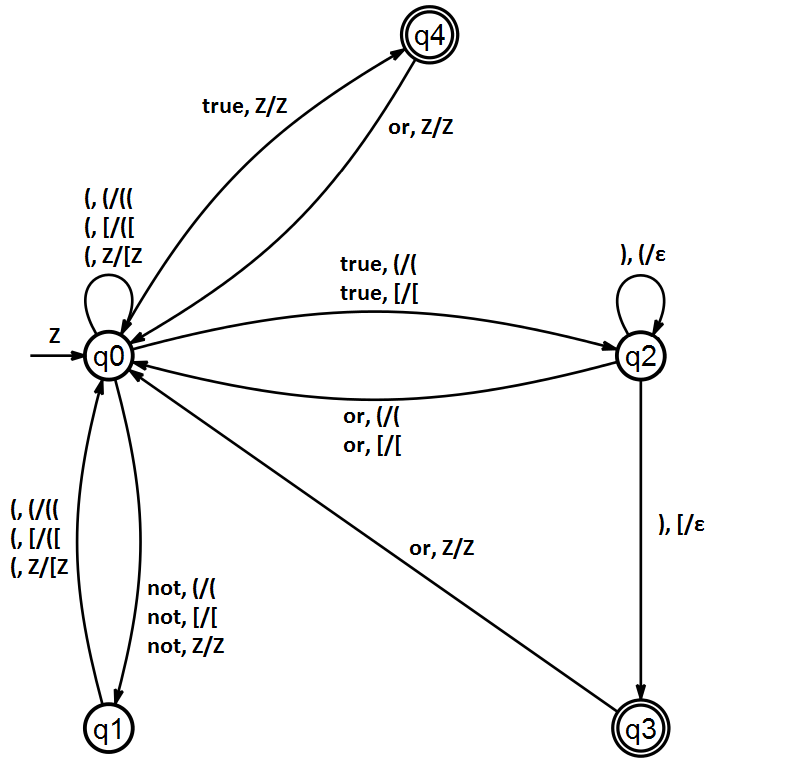
\includegraphics{img/dza2.png}
        }
        \end{center}
        \end{figure}

  \newpage

  DZA $M_2$ přijímající doplněk jazyka $L_{4}$ získáme z DZA $M_1$ záměnou koncových a nekoncových stavů a přidáním sink stavu.\\\\
$M_2 = (Q_{2}, \Sigma_{2}, \Gamma_{2}, \delta_{2}, q_{0}, Z, F_{2})$, kde:
  \begin{eqnarray*}
    Q_{2}&=&\{q_{0}, q_{1}, q_{2}, q_{3}, q_{4}, q_{5}\}\\
   \Sigma_{2}&=&\{(,),true,or,not\}\\
   \Gamma_{2}&=&\{Z,(,[\}\\
    F_{2}&=&\{q_{0}, q_{1}, q_{2}, q_{5}\}
  \end{eqnarray*}

  Přechodovou funkci $\delta_{2}$ znázorňuje diagram:\\

\begin{figure}[h!]
        \begin{center}
        \scalebox{0.5}{
        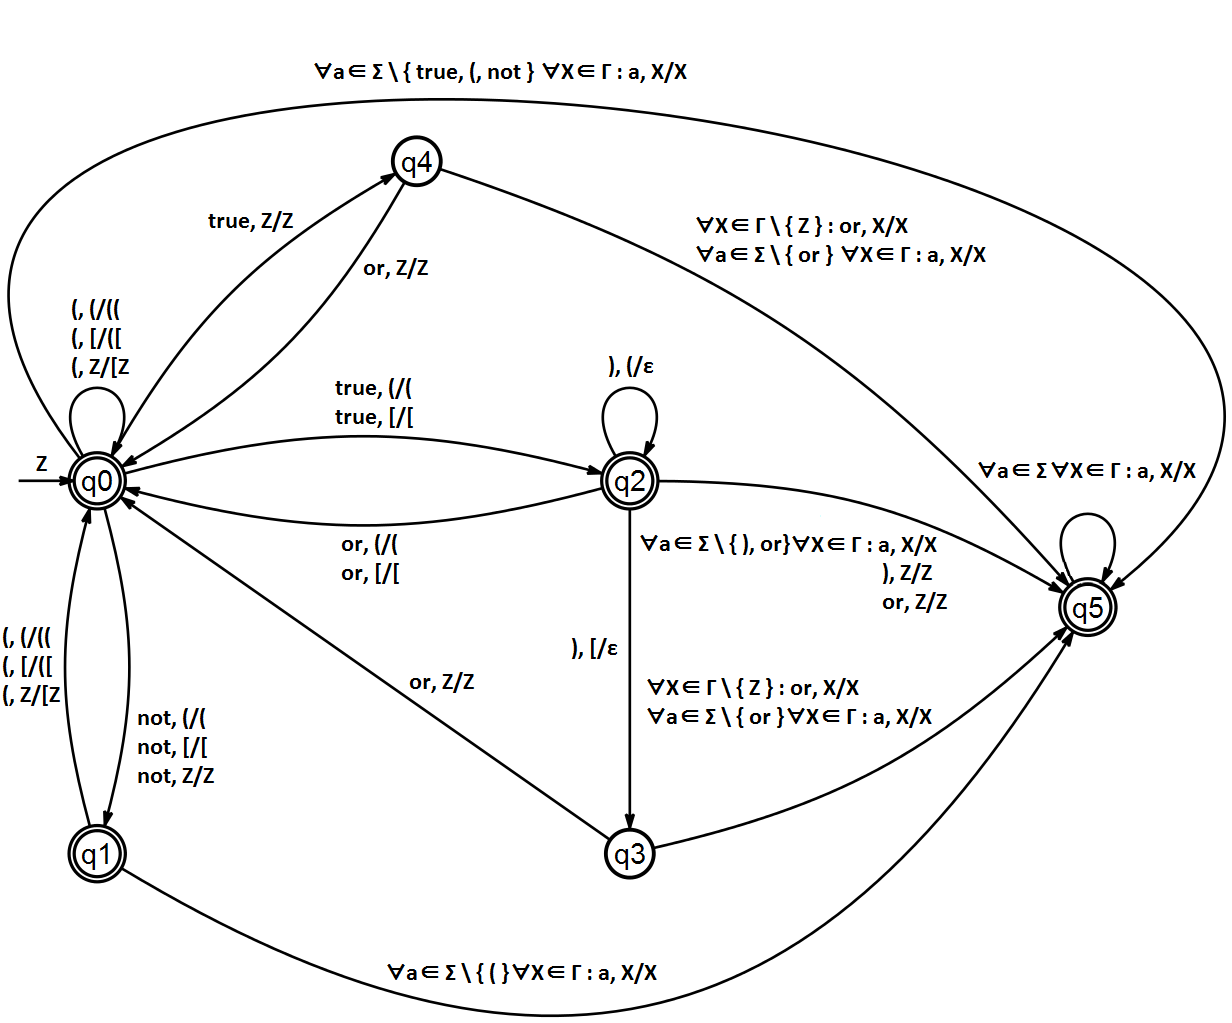
\includegraphics{img/dzas.png}
        }
        \end{center}
        \end{figure}

  \newpage

  Pro vstupní řezězec $(true \: or \: not(true)) \: or \: true$ realizuje automat $M_2$ tyto přechody:

  \begin{eqnarray*}
  (q_{0}, (true \: or \: not(true)) \: or \: true, Z)&\vdash&(q_{0}, true \: or \: not(true)) \: or \: true, [Z)\\
  &\vdash&(q_{2}, or \: not(true)) \: or \: true, [Z)\\
  &\vdash&(q_{0}, not(true)) \: or \: true, [Z)\\
  &\vdash&(q_{1}, (true)) \: or \: true, [Z)\\
  &\vdash&(q_{0}, true)) \: or \: true, ([Z)\\
  &\vdash&(q_{2}, )) \: or \: true, ([Z)\\
  &\vdash&(q_{2}, ) \: or \: true, [Z)\\
  &\vdash&(q_{3}, or \: true, Z)\\
  &\vdash&(q_{0}, true, Z)\\
  &\vdash&(q_{4}, \epsilon, Z)\\
  \end{eqnarray*}

  Automat se po přečtení celého řetězce nachází v nekoncovém stavu, tento řetězec tedy nebyl automatem přijat. 

  \newpage

\newpage

\item Mějme gramatiku $G_{5}=(\{S,A,B\},\{a,b,c\},P,S)$, kde

\begin{eqnarray*}
      P: \:\:\:\:\:\:\:\:\:\:\: S&\rightarrow&aABa\\
      A&\rightarrow&B \mid a \mid c\\
      B&\rightarrow&Bc \mid bB \mid \epsilon\\
\end{eqnarray*}

Převeďte gramatiku $G_{5}$ \emph{algoritmicky} do (a) Chomského normální formy a (b) Greibachové normální formy.\\

Nejprve převedeme gramatiku  $G_{5}$ na ekvivalentní vlastní gramatiku odstraněním $\epsilon$-pravidel, zbytečných symbolů a cyklů, přičemž cykly odstraníme odstraněním $\epsilon$-pravidel a jednoduchých pravidel:
    \begin{itemize}
      \item Převod gramatiky $G_{5}$ na ekvivalentní gramatiku bez $\epsilon$-pravidel $G_{6}$ s pomocí algoritmu \textbf{4.4} ze studijní opory:\\\\
      Krok (1):\\\\
      $N_{0} = \emptyset$\\
      $N_{1} = \{A \mid A \rightarrow \alpha \in P \wedge \alpha \in (N_{0} \cup \epsilon)^{*}\} \cup N_{0} = \{B\}$\\
      $N_{2} = \{A \mid A \rightarrow \alpha \in P \wedge \alpha \in (N_{1} \cup \epsilon)^{*}\} \cup N_{1} = \{A,B\}$\\
      $N_{3} = \{A \mid A \rightarrow \alpha \in P \wedge \alpha \in (N_{2} \cup \epsilon)^{*}\} \cup N_{2} = \{A,B\} = N_{2} = N_{\epsilon}$\\\\
      Krok (2a): \\\\
      Do nové množiny přepisovacích pravidel $P_{6}$ přidáme:
      \begin{eqnarray*}
      S&\rightarrow&aABa \mid aBa \mid aAa \mid aa\\
      A&\rightarrow&B \mid a \mid c\\
      B&\rightarrow&Bc \mid bB \mid c \mid b\\
      \end{eqnarray*}
      Krok (2b): \\\\
      Protože $S \notin N_{\epsilon}$, množina neterminálů i počáteční symbol gramatiky $G_{6}$ jsou stejné jako u gramatiky $G_{5}$.\\\\
      Krok (3): \\\\
      Výsledná gramatika bez $\epsilon$-pravidel:\\\\ $G_{6} = (\{S,A,B\},\{a,b,c\},P_{6},S)$, kde:
      \begin{eqnarray*}
      P_{6}: \:\:\:\:\:\:\:\:\:\:\: S&\rightarrow&aABa \mid aBa \mid aAa \mid aa\\
      A&\rightarrow&B \mid a \mid c\\
      B&\rightarrow&Bc \mid bB \mid c \mid b\\
      \end{eqnarray*}
      \newpage
      \item Převod gramatiky bez $\epsilon$-pravidel $G_{6}$ na ekvivalentní gramatiku bez $\epsilon$-pravidel a bez jednoduchých pravidel  $G_{7}$ s pomocí algoritmu \textbf{4.5} ze studijní opory:\\\\
      Krok (1):\\\\
     $N_{0} = \{S\}$\\
     $N_{1} = \{C \mid B \rightarrow C \in P_{6} \wedge B \in N_{0}\} \cup N_{0} = \{S\}$\\
     $N_{1} = N_{0},  N_{S} = N_{1} = \{S\}$\\\\
     $N_{0} = \{A\}$\\
     $N_{1} = \{C \mid B \rightarrow C \in P_{6} \wedge B \in N_{0}\} \cup N_{0} = \{A,B\}$\\
     $N_{1} \neq N_{0}$\\
     $N_{2} = \{C \mid B \rightarrow C \in P_{6} \wedge B \in N_{1}\} \cup N_{1} = \{A,B\}$\\
     $N_{2} = N_{1},  N_{A} = N_{2} = \{A,B\}$\\\\
     $N_{0} = \{B\}$\\
     $N_{1} = \{C \mid B \rightarrow C \in P_{6} \wedge B \in N_{0}\} \cup N_{0} = \{B\}$\\
     $N_{1} = N_{0},  N_{B} = N_{1} = \{B\}$\\\\
      Krok (2):\\
      \begin{eqnarray*}
      P_{7}: \:\:\:\:\:\:\:\:\:\:\: S&\rightarrow&aABa \mid aBa \mid aAa \mid aa\\
      A&\rightarrow&Bc \mid bB \mid a \mid c \mid b\\
      B&\rightarrow&Bc \mid bB \mid c \mid b\\
      \end{eqnarray*}
      Krok (3):\\\\
      Výsledná gramatika bez $\epsilon$-pravidel a jednoduchých pravidel:\\\\ $G_{7} = (\{S,A,B\},\{a,b,c\},P_{7},S)$.\\
      \newpage
      \item Převod gramatiky bez $\epsilon$-pravidel a jednoduchých pravidel $G_{7}$ na ekvivalentní gramatiku bez $\epsilon$-pravidel, jednoduchých pravidel a zbytečných symbolů (a tedy vlastní gramatiku) $G_{8}$ s pomocí algoritmu \textbf{4.3} ze studijní opory:\\\\
      Krok (1):\\\\
      $N_{0} = \emptyset$\\
      $N_{1} = \{A \mid A \rightarrow \alpha \in P_{7} \wedge \alpha \in (N_{0} \cup \Sigma)^{*}\} \cup N_{0} = \{S,A,B\}$\\
      $N_{2} = \{A \mid A \rightarrow \alpha \in P_{7} \wedge \alpha \in (N_{1} \cup \Sigma)^{*}\} \cup N_{1} = \{S,A,B\} = N_{1} =  N_{t}$\\\\
      $\overline{G_{7}} = (\{S,A,B\}, \{a,b,c\},\overline{P_{7}},S)$, kde:\\
     \begin{eqnarray*}
      \overline{P_{7}}: \:\:\:\:\:\:\:\:\:\:\: S&\rightarrow&aABa \mid aBa \mid aAa \mid aa\\
      A&\rightarrow&Bc \mid bB \mid a \mid c \mid b\\
      B&\rightarrow&Bc \mid bB \mid c \mid b\\
     \end{eqnarray*}
      Krok (2):\\\\
      $V_{0} = \{S\}$\\
      $V_{1} = \{X \mid A \rightarrow \alpha X \beta \in \overline{P_{7}} \wedge A \in V_{0}\} \cup V_{0} = \{S,A,B,a\}$\\
      $V_{2} = \{X \mid A \rightarrow \alpha X \beta \in \overline{P_{7}} \wedge A \in V_{1}\} \cup V_{1} = \{S,A,B,a,b,c\}$\\
      $V_{3} = \{X \mid A \rightarrow \alpha X \beta \in \overline{P_{7}} \wedge A \in V_{2}\} \cup V_{2} = \{S,A,B,a,b,c\} = V_{2}$\\\\
      Výsledná vlastní gramatika:\\\\$G_{8}=(N_{8}, \Sigma_{8},P_{8},S)$, kde:
      \begin{eqnarray*}
        N_{8}&=&V_{3} \cap \{S,A,B\}=\{S,A,B\}\\
        \Sigma_{8}&=&V_{3} \cap \{a,b,c\}=\{a,b,c\}
      \end{eqnarray*}
      \begin{eqnarray*}
      P_{8}: \:\:\:\:\:\:\:\:\:\:\: S&\rightarrow&aABa \mid aBa \mid aAa \mid aa\\
      A&\rightarrow&Bc \mid bB \mid a \mid c \mid b\\
      B&\rightarrow&Bc \mid bB \mid c \mid b\\
     \end{eqnarray*}
    \end{itemize}

    \newpage
    \renewcommand{\theenumi}{\alph{enumi}}
    \begin{enumerate}
      \item Převod vlastní gramatiky $G_{8}$ na ekvivalentní gramatiku $G_{G}$ v Greibachové normální formě.\\

      Nejprve musíme vlastní gramatiku $G_{8}$ převést na ekvivalentní vlastní gramatiku bez levé rekurze $G_{9}$ s použitím algoritmu \textbf{4.6} ze studijní opory:\\\\
      Krok (1): Položme $A_{1} = S$, $A_{2} = A$, $A_{3} = B$, $i = 1$, $n = 3$ \\
      Krok (2): beze změny\\
      Krok (3): $i \neq n$, takže položíme $i = i+1=2$, $j = 1$\\
      Krok (4): beze změny\\
      Krok (5): $j = i-1$, takže přejdeme na krok (2)\\
      Krok (2): beze změny\\
      Krok (3): $i \neq n$, takže položíme $i = i+1=3$, $j = 1$\\
      Krok (4): beze změny\\
      Krok (5): $j \neq i-1$, takže položíme $j = j+1=2$ a přejdeme na krok (4)\\
      Krok (4): beze změny\\
      Krok (5): $j = i-1$, takže přejdeme na krok (2)\\
      Krok (2): Nahradíme pravidla:
      \begin{eqnarray*}
        B&\rightarrow&Bc \mid bB \mid c \mid b\\
        &\downarrow&\\
        B&\rightarrow&bB \mid c \mid b \mid bBB' \mid cB' \mid bB'\\
        B'&\rightarrow&c \mid cB'\\
      \end{eqnarray*}
      Krok (3): \\\\$i = n$, získali jsme výslednou vlastní gramatiku bez levé rekurze:\\\\ $G_{9} = (\{S,A,B,B'\}, \{a,b,c\},P_{9},S)$, kde:
      \begin{eqnarray*}
      P_{9}: \:\:\:\:\:\:\:\:\:\:\: S&\rightarrow&aABa \mid aBa \mid aAa \mid aa\\
      A&\rightarrow&Bc \mid bB \mid a \mid c \mid b\\
      B&\rightarrow&bB \mid c \mid b \mid bBB' \mid cB' \mid bB'\\
      B'&\rightarrow&c \mid cB'\\
      \end{eqnarray*}
     
      \newpage
      Nyní převedeme vlastní gramatiku bez levé rekurze $G_{9}$ na ekvivalentní gramatiku $G_{G}$ v Greibachové normální formě s pomocí algoritmu \textbf{4.8} ze studijní opory:\\\\
      Krok (1): $S < A < B < B'$, $n=4$\\
      Krok (2): Položíme $i = n - 1 = 3$\\
      Krok (3): $i \neq 0$, není co nahradit\\
      Krok (4): Položíme $i = i - 1 = 2$, pokračujeme krokem (3)\\
      Krok (3): $i \neq 0$, nahradíme pravidlo:
      \begin{eqnarray*}
        A&\rightarrow&Bc\\
        &\downarrow&\\
        A&\rightarrow&bBc \mid cc \mid bc \mid bBB'c \mid cB'c \mid bB'c
      \end{eqnarray*}
      Krok (4): Položíme $i = i - 1 = 1$, pokračujeme krokem (3)\\
      Krok (3): $i \neq 0$, není co nahradit\\
      Krok (4): Položíme $i = i - 1 = 0$, pokračujeme krokem (3)\\
      Krok (3): $i = 0$, pokračujeme krokem (5)\\
      Krok (5): nahradíme pravidla:
      \begin{eqnarray*}
       S&\rightarrow&aABa \mid aBa \mid aAa \mid aa\\
       A&\rightarrow&bBc \mid cc \mid bc \mid bBB'c \mid cB'c \mid bB'c\\
        &\downarrow&\\
       S&\rightarrow&aABA' \mid aBA' \mid aAA' \mid aA'\\
       A&\rightarrow&bBC' \mid cC' \mid bC' \mid bBB'C' \mid cB'C' \mid bB'C'
      \end{eqnarray*}
      Krok (6): přidáme pravidla:
      \begin{eqnarray*}
        A'&\rightarrow&a\\
        C'&\rightarrow&c\\
      \end{eqnarray*}
      %\newpage
      Výsledná gramatika v Greibachové normální formě:\\\\$G_{G} = (\{S,A,A',B,B',C'\}, \{a,b,c\},P_{G},S)$, kde:
      \begin{eqnarray*}
      P_{G}: \:\:\:\:\:\:\:\:\:\:\: S&\rightarrow&aABA' \mid aBA' \mid aAA' \mid aA'\\
      A&\rightarrow&bBC' \mid cC' \mid bC' \mid bBB'C' \mid cB'C' \mid bB'C' \mid bB \mid a \mid c \mid b\\
      A'&\rightarrow&a\\
      B&\rightarrow&bB \mid c \mid b \mid bBB' \mid cB' \mid bB'\\
      B'&\rightarrow&c \mid cB'\\
      C'&\rightarrow&c\\
      \end{eqnarray*}
      \newpage

      \item Převod vlastní gramatiky bez jednoduchých pravidel $G_{8}$ na ekvivalentní gramatiku $G_{CH}$ v Chomského normální formě s pomocí algoritmu \textbf{4.7} ze studijní opory:\\

      Krok (1): $P_{CH}$ obsahuje pravidla:
     \begin{eqnarray*}
      A&\rightarrow&a \mid c \mid b\\
      B&\rightarrow&c \mid b
      \end{eqnarray*}
      Krok (2): beze změny\\
      Krok (3): beze změny\\
      Krok (4):\\
      \begin{minipage}{.3\linewidth}
      \begin{eqnarray*}
       S&\rightarrow&aABa\\
        &\downarrow&\\
       S&\rightarrow&a' \langle ABa \rangle\\
       \langle ABa \rangle&\rightarrow&A\langle Ba \rangle\\
       \langle Ba \rangle&\rightarrow&Ba'\\
      \end{eqnarray*}
      \end{minipage}%
      \begin{minipage}{.3\linewidth}
      \begin{eqnarray*}
       S&\rightarrow&aBa\\
        &\downarrow&\\
       S&\rightarrow&a' \langle Ba \rangle\\
       \langle Ba \rangle&\rightarrow&Ba'\\
      \end{eqnarray*}
      \end{minipage}
      \begin{minipage}{.3\linewidth}
      \begin{eqnarray*}
       S&\rightarrow&aAa\\
        &\downarrow&\\
       S&\rightarrow&a' \langle Aa \rangle\\
       \langle Aa \rangle&\rightarrow&Aa'\\
      \end{eqnarray*}
      \end{minipage}

      Krok (5):\\
      \begin{minipage}{.2\linewidth}
      \begin{eqnarray*}
       S&\rightarrow&aa\\
        &\downarrow&\\
       S&\rightarrow&a'a'\\
      \end{eqnarray*}
      \end{minipage}%
      \begin{minipage}{.2\linewidth}
      \begin{eqnarray*}
       A&\rightarrow&Bc\\
        &\downarrow&\\
       A&\rightarrow&Bc'\\
      \end{eqnarray*}
      \end{minipage}
      \begin{minipage}{.2\linewidth}
      \begin{eqnarray*}
       A&\rightarrow&bB\\
        &\downarrow&\\
       A&\rightarrow&b'B\\
      \end{eqnarray*}
      \end{minipage}
      \begin{minipage}{.2\linewidth}
      \begin{eqnarray*}
       B&\rightarrow&Bc\\
        &\downarrow&\\
       B&\rightarrow&Bc'\\
      \end{eqnarray*}
      \end{minipage}%
      \begin{minipage}{.2\linewidth}
      \begin{eqnarray*}
       B&\rightarrow&bB\\
        &\downarrow&\\
       B&\rightarrow&b'B\\
      \end{eqnarray*}
      \end{minipage}

      Krok (6): Do $P_{CH}$ přidáme pravidla:
      \begin{eqnarray*}
       a'&\rightarrow&a\\
       b'&\rightarrow&b\\
       c'&\rightarrow&c\\
      \end{eqnarray*}

       %\newpage

        Výsledná gramatika v Chomského normální formě:\\\\$G_{CH} = (\{S,A,B,\langle ABa \rangle, \langle Ba \rangle, \langle Aa \rangle, a',b',c'\}, \{a,b,c\},P_{CH},S)$, kde:\\
      \begin{eqnarray*}
        P_{CH}: \:\:\:\:\:\:\:\:\:\:\: S&\rightarrow&a' \langle ABa \rangle \mid a' \langle Ba \rangle \mid a' \langle Aa \rangle \mid a'a'\\
        A&\rightarrow&a \mid c \mid b \mid Bc' \mid b'B\\
        B&\rightarrow&c \mid b \mid Bc' \mid b'B\\
       \langle ABa \rangle&\rightarrow&A\langle Ba \rangle\\
       \langle Ba \rangle&\rightarrow&Ba'\\
       \langle Aa \rangle&\rightarrow&Aa'\\
       a'&\rightarrow&a\\
       b'&\rightarrow&b\\
       c'&\rightarrow&c\\
      \end{eqnarray*}

    \end{enumerate}
    \renewcommand{\theenumi}{\arabic{enumi}}



\end{enumerate}






\end{document}